\documentclass[a4paper, 12pt]{article}

\usepackage{hyperref}
\usepackage[warn]{mathtext}
\usepackage[utf8]{inputenc}
\usepackage[T2A]{fontenc}
\usepackage[english,russian]{babel}
\usepackage{multirow}
\usepackage{amsmath,amsfonts,amssymb,amsthm,mathtools}
\usepackage{indentfirst}
\DeclareSymbolFont{T2Aletters}{T2A}{cmr}{m}{it}
\usepackage{ gensymb }
\mathtoolsset{showonlyrefs=true}
\usepackage{euscript}
\usepackage{mathrsfs}
\usepackage[left=2cm,right=2cm,top=2cm,bottom=2cm]{geometry}
\usepackage{graphicx}
\usepackage{wrapfig}
\usepackage[rgb]{xcolor}
\hypersetup{
colorlinks=true,
urlcolor=blue
}


\title{Лабораторная работа}
\author{Гисич Арсений Б03-102}
\date{2022}

\begin{document}

	\begin{center}
		{\large МОСКОВСКИЙ ФИЗИКО-ТЕХНИЧЕСКИЙ ИНСТИТУТ (НАЦИОНАЛЬНЫЙ ИССЛЕДОВАТЕЛЬСКИЙ УНИВЕРСИТЕТ)}
	\end{center}
	\vspace{5 cm}
	{\Large
		\begin{center}
			{\bf Лабораторная работа 3.3.4}\\[0.2 cm]
			Эффект Холла в полупроводниках
		\end{center}
	}
	\vspace{4 cm}
	\begin{flushright}
		{\Large Выполнил: \\
			\vspace{0.2 cm}
			Гисич Арсений \\
			\vspace{0.2 cm}
			Б03-102 \\}
	\end{flushright}
	\vspace{9 cm}
	\begin{center}
		Долгопрудный\\[0.1 cm]
		2022
	\end{center}
\thispagestyle{empty}

\section{Аннотация}

В данной работе исследовалась зависимость ЭДС Холла от величины магнитного поля при различных значениях тока через образец для определения константы Холла. Также был определён знак носителей заряда и проводимость материала образца.

\section{Теоретические сведения}

Суть эффекта Холла состоит в следующем. Пусть через однородную пластину металла вдоль оси $x$ течет ток $I$ (рис.~\ref{ris1}).
	
\begin{wrapfigure}{l}{0.6\textwidth}
	\vspace{-20pt}
	\begin{center}
		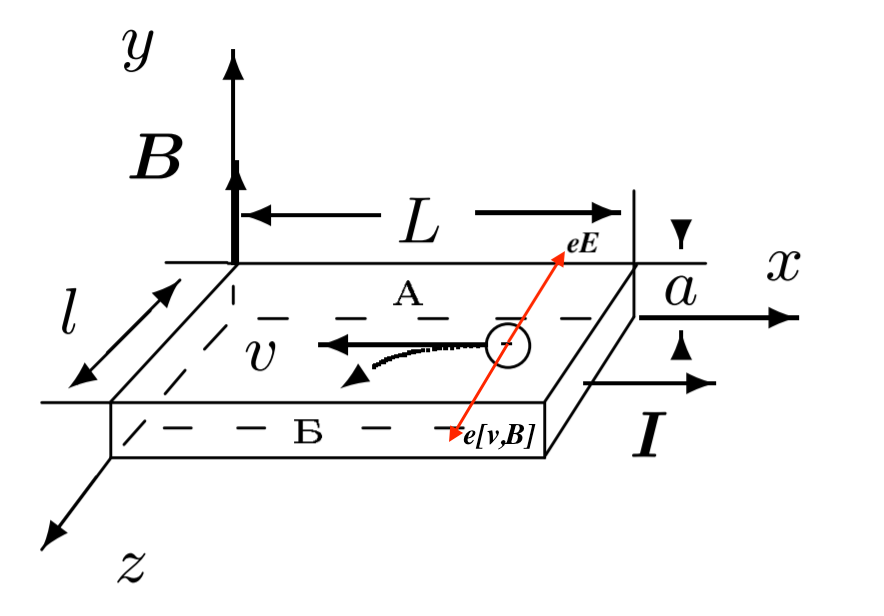
\includegraphics[width=0.7\linewidth]{1.png}
		\label{ris1}
	\end{center}
	\vspace{-20pt}
	\caption{Образец с током в магнитном поле}
\end{wrapfigure}

	Если эту пластину поместить в магнитное поле, направленное по оси y, то между гранями А и Б появляется разность потенциалов. 
	
	В самом деле, на электрон (для простоты рассматриваем один тип носителей), движущийся со средней скоростью $\langle \vec{v} \rangle$ в электромагнитном поле, действует сила Лоренца:
	
	$$\vec{F}_{л} = -e\vec{E}-e \langle \vec{v} \rangle \times \vec{B},$$
	
	где $e$ --- абсолютный заряд электрона, $\vec{E}$ --- напряженность электрического поля, $\vec{B}$ --- индукция магнитного поля.
	
	В проекции на ось $z$ получаем
	
	$$ F_{B}=e | \langle {v_{x}} \rangle | B.$$
	
	Под действием этой силы электроны отклоняются к грани Б, заряжая ее отрицательно. На грани А накапливаются нескомпенсированные положительные заряды. Это приводит к возникновению электрического поля $E_{z}$, направленного от А к Б, которое действует на электроны с силой $F_{E}=eE_{z}$. В установившемся режиме $F_{E}=F_{B}$, поэтому накопление электрических зарядов на боковых гранях пластины прекращается. Отсюда
	
	$$ E_{z}=| \langle {v_{x}} \rangle | B.$$
	
	С этим полем связана разность потенциалов $$U_{AБ}=E_{z}l=| \langle {v_{x}} \rangle | Bl.$$
	
	В этом и состоит эффект Холла.
	
	\
	
	Замечая, что сила тока
	
	$$ I=ne| \langle {v_{x}} \rangle |la,$$
	
	найдем ЭДС Холла:
	
\begin{equation}\label{Rx}
	\mathscr{E}_{X}=U_{AБ}=\dfrac{IB}{nea}=R_{X}\dfrac{IB}{a}.
\end{equation}
	
	Константа $R_{X}=\dfrac{1}{ne}$ называется постоянной Холла.
	
	В полупроводниках, когда вклад в проводимость обусловлен и электронами и дырками, выражение для постоянной Холла имеет более сложный вид:
	
	$$R_{X}=\dfrac{nb^{2}_{e}-pb^{2}_{p}}{e(nb_{e}+pb_{p})^{2}},$$
	
	где $n$ и $p$ --- концентрации электронов и дырок; $b_{e}$, $b_{p}$ --- их подвижности.

\section{Методика измерений}

Схема экспериментальной установки показана на рис.~\ref{ris2}.
	
\begin{figure}[h!]
\begin{center}
    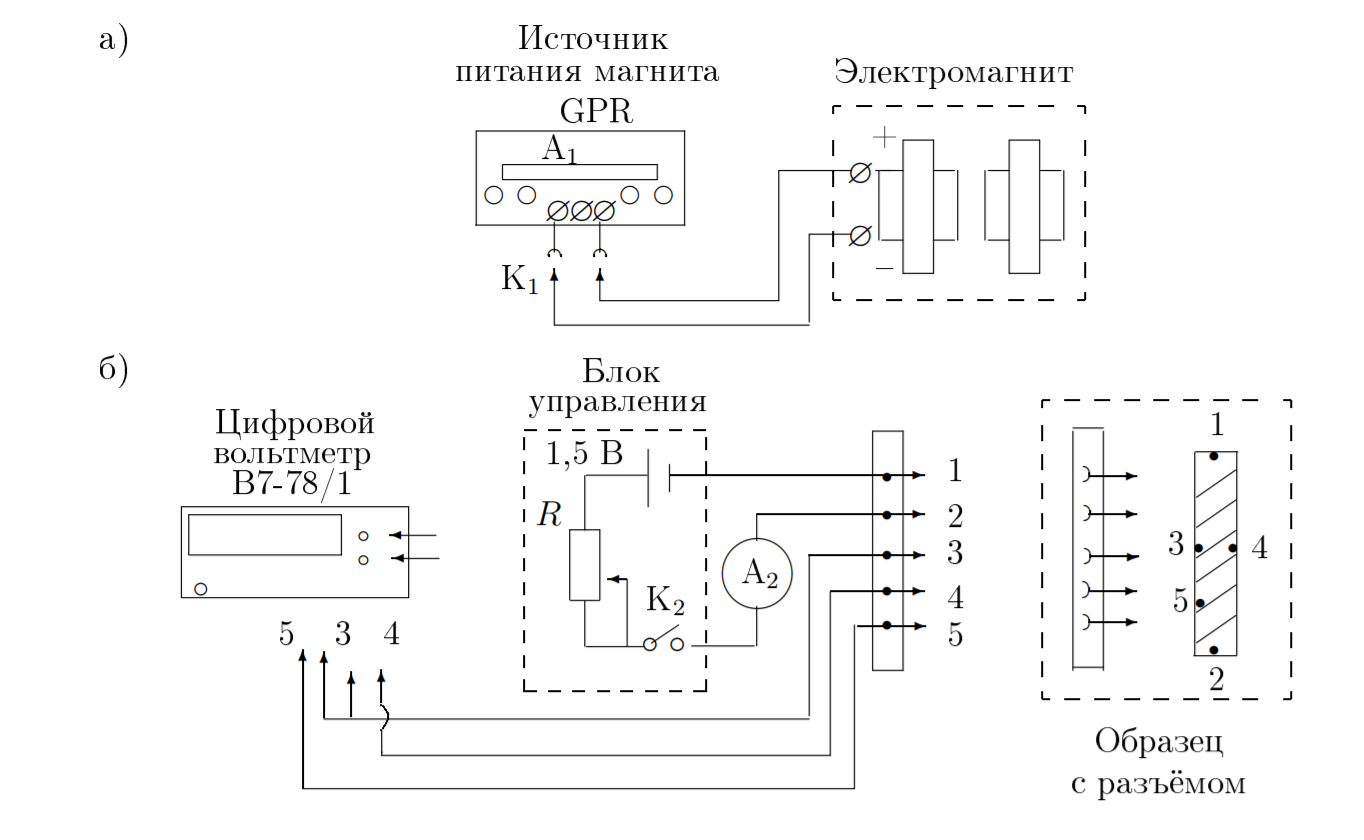
\includegraphics[width=\linewidth]{2.png}
\end{center}
\caption{Схема установки для исследования эффекта Холла в полупроводниках}
\label{ris2}
\end{figure}
  
  	В зазоре электромагнита (рис.~\ref{ris2}a) создаётся постоянное магнитное поле, величину которого можно менять с помощью регуляторов источника питания. Ток измеряется амперметром источника питания $A_{1}$. Разъем $K_{1}$ позволяет менять направление тока в обмотках электромагнита.
  
  	Образец из легированного германия, смонтированный в специальном держателе (рис.~\ref{ris2}б), подключается к батарее. При замыкании ключа $K_{2}$ вдоль длинной стороны образца течет ток, величина которого регулируется реостатом $R$ и измеряется миллиамперметром $А_{2}$.
  	
  	В образце с током, помещённом в зазор электромагнита, между контактами 3 и 4 возникает разность потенциалов $U_{34}$, которая измеряется с помощью цифрового вольтметра.
  	
  	Контакты 3 и 4 вследствие неточности подпайки не всегда лежат на одной
  	эквипотенциали, и тогда напряжение между ними связано не только с эффектом
  	Холла, но и с омическим падением напряжения, вызванным протеканием основного тока через образец.
  	
  	Измеряемая разность потенциалов при одном направлении
  	магнитного поля равна сумме ЭДС Холла и омического падения напряжения, а
  	при другом  их разности. В этом случае ЭДС Холла $\mathscr{E}_{X}$ может быть определена как половина алгебраической разности показаний вольтметра, полученных для
  	двух противоположных направлений магнитного поля в зазоре.
  	
  	Можно исключить влияние омического падения напряжения иначе, если при каждом токе через образец измерять напряжение между точками 3 и 4 в отсутствие магнитного поля. При фиксированном токе через образец это дополнительное к ЭДС Холла напряжение $U_{0}$ остается неизменным. От него следует (с учетом
  	знака) отсчитывать величину ЭДС Холла: 
  	
  	$$\mathscr{E}_{X} = U_{34} - U_{0}.$$
  	
  	При таком способе измерения нет необходимости проводить повторные измерения с противоположным направлением магнитного поля.
  	
  	
  	По знаку $\mathscr{E}_{X}$ можно определить характер проводимости --- электронный или дырочный. Для этого необходимо знать направление тока в образце и направление
  	магнитного поля.
  	
  	Измерив ток $I$ в образце и напряжение $U_{35}$ между контактами 3 и 5 в отсутствие магнитного поля, можно, зная параметры образца, рассчитать проводимость материала образца по формуле:
  	
  \begin{equation}\label{sigma}
  	\sigma=\dfrac{IL_{35}}{U_{35}ah},
  \end{equation}
  	
где $L_{35}$ --- расстояние между контактами 3 и 5, $a$ --- толщина образца, $h$ --- его толщина.
  	
\section{Используемое оборудование}

\begin{enumerate}
    \item электромагнит с регулируемым источником питания;
    \item вольтметр;
    \item амперметр;
    \item миллиамперметр;
    \item милливеберметр или миллитесламетр;
    \item источник питания;
    \item образцы легированного германия;
\end{enumerate}

\section{Результаты измерений и обработка данных}


\begin{table}[h!]
\begin{center}
\begin{tabular}{|c|c|c|c|c|c|}
\hline
$\tau, мкс$ & $\delta_{\tau}, мкс$ & $T, \celsius$ & $\delta_T, \celsius$ & $\Delta{U}, мВ$ & $\delta_{\Delta{U}}, мВ$ \\ \hline
10,068 & 0,001 & 14,04 & 0,01 & -0,012 & 0,001 \\ \hline
9,955 & 0,001 & 16,03 & 0,01 & -0,017 & 0,001 \\ \hline
9,753 & 0,001 & 18,03 & 0,01 & -0,014 & 0,001 \\ \hline
9,433 & 0,001 & 20,03 & 0,01 & -0,015 & 0,001 \\ \hline
9,042 & 0,001 & 22,01 & 0,01 & -0,016 & 0,001 \\ \hline
8,747 & 0,001 & 24,02 & 0,01 & -0,017 & 0,001 \\ \hline
8,609 & 0,001 & 26,01 & 0,01 & -0,017 & 0,001 \\ \hline
8,534 & 0,001 & 28,01 & 0,01 & -0,015 & 0,001 \\ \hline
8,488 & 0,001 & 30,00 & 0,01 & -0,017 & 0,001 \\ \hline
8,453 & 0,001 & 32,00 & 0,01 & -0,017 & 0,001 \\ \hline
8,429 & 0,001 & 34,00 & 0,01 & -0,018 & 0,001 \\ \hline
8,409 & 0,001 & 36,01 & 0,01 & -0,016 & 0,001 \\ \hline
8,395 & 0,001 & 38,00 & 0,01 & -0,016 & 0,001 \\ \hline
8,383 & 0,001 & 40,00 & 0,01 & -0,017 & 0,001 \\ \hline
\end{tabular}
\end{center}
\caption{Результаты измерения зависимости периода колебаний $LC$-генератора от температуры образца}
\label{tab1}
\end{table}


\section{Обсуждение результатов и выводы}

В данной работе была исследована температурная зависимость магнитной восприимчивости гадолиния выше точки Кюри. Также была рассчитана парамагнитная точка Кюри для данного металла.

Полученное значение парамагнитной точки Кюри: $$\boxed{\Theta_p = 17,96\pm0,03~\celsius}$$
Данное значение существенно отличается от табличного (20,2~\textcelsius). Основной вклад в погрешность вносит погрешность определения температуры образца. Расхождение может быть вызвано неравномерным нагревом установки и сосуда с образцом. Как и предполагалось законом Кюри-Вейсса, данная температура выше ферромагнитной точки Кюри, которая равна 16~\textcelsius{}. Также, данное значение согласуется с оценочным, полученным из графика.

\end{document}
